\subsection{Einfluss des Verstärkers}
Ein unverstärkter Puls ist in Abbildung \ref{fig:unverstaerkt} abgebildet.
Die Abklingzeit $τ$ beträgt
\begin{align}
    τ &= \SI{50}{\micro\second} \\
    p &= \SI{0.068}{\milli\bar} \\
    φ &= \SI{0}{\degree}\:.
\end{align}
Für die Abbildung \ref{fig:verstaerkt} wurde ein Nachleuchten von
$\SI{5}{\second}$ eingestellt. Die Abklingzeit ist deutlich kürzer mit
\begin{align}
    τ &= \SI{1}{\micro\second} \\
    p &= \SI{0.054}{\milli\bar} \\
    φ &= \SI{0}{\degree}\:.
\end{align}
\begin{figure}
    \centering
    \caption{Pulse auf dem Oszilloskopschirm.}
    \begin{subfigure}{0.49\textwidth}
        \centering
        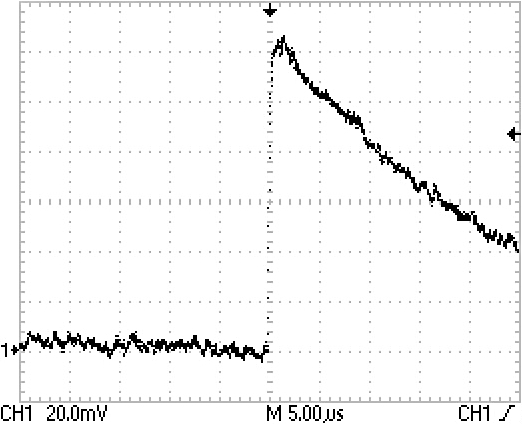
\includegraphics[width=0.9\textwidth]{images/unverstaerkt.JPG}
        \caption{Unverstärkter Puls auf dem Oszilloskopschirm.}
        \label{fig:unverstaerkt}
    \end{subfigure}
    \begin{subfigure}{0.49\textwidth}
        \centering
        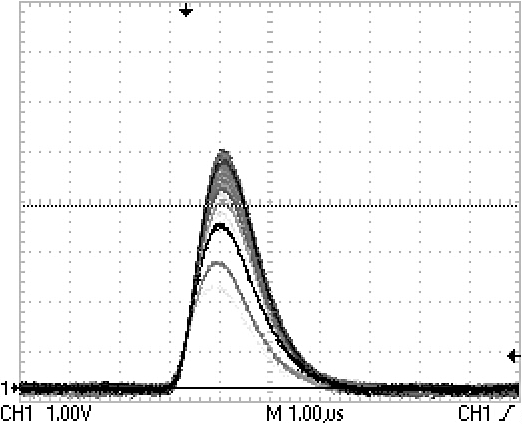
\includegraphics[width=0.9\textwidth]{images/verstaerkt.JPG}
        \caption{Verstärkte Pulse auf dem Oszilloskopschirm.}
        \label{fig:verstaerkt}
    \end{subfigure}
\end{figure}

Es kann dabei sehr gut beobachtet werden, dass der Verstärker die Peakhöhe
von circa $\SI{124}{\milli\volt}$ im unverstärkten Signal zu
$\SI{5}{\volt}$ verstärkt wird.
Ohne die Verstärkung startet der Puls instantan. Die Verstärkung
verschmiert auß\,erdem das Signal in die Breite.
